This section provides an overview of The Smart Shutter. The primary operational aspects of our product, from the perspective of end users, maintainers and administrators, are defined here. The key features and functions found in the product, as well as critical user interactions and user interfaces are described in detail

\subsection{Features \& Functions}
The Smart Shutters main functionality is to change position remotely according to the users, who will either set a schedule for the shutters to follow or real time user input. The users will interact with the shutters through an app that is available on either android or ios. The app will then communicate to a hub that will then relay the request to each shutter. 


\subsection{External Inputs \& Outputs}
From the users we expect positions, meaning either preset positions or a specific number for how much light the shutter should let in. From the system we expect a few outputs such as an acknowledgement for receiving the request and completed the request, then it will state the new position of the shutters and the battery level. 

\subsection{Product Interfaces}
\begin{figure}[H]
    \centering
    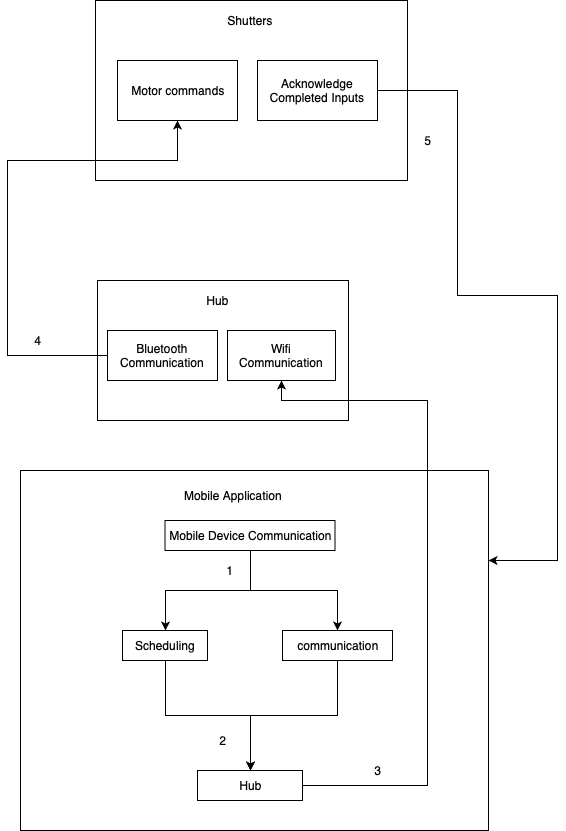
\includegraphics[width=0.5\textwidth]{images/SystemOverview}
    \caption{System Overview}
\end{figure}
